\section{Experimental Design}
\label{sec:setup}

\subsection{Benchmark Transit Corridors and Empirical MBTA Reconstruction}
\label{sec:setup_corridors}

To evaluate \texttt{FreqDuet} across controlled non-stationary regimes, empirical urban operations, and stationary null conditions, we construct three bidirectional fixed-pool corridor benchmarks operating from $06{:}00$ to $19{:}03$ ($T_{\mathrm{end}} = 46{,}980\text{ s}$) with a $4\text{-h}$ clearance horizon ($T_{\mathrm{eval}} = 61{,}380\text{ s}$) and stochastic link speeds ($\sigma_{\mathrm{route}} = 1.5\text{ m/s}$), day-level demand noise ($\pm 15\%$), and CRN-synchronized $15\text{-min}$ localized station surges ($4$ surges/day, $1.5\times$--$2.4\times$ local boarding intensity across $3$ adjacent stops):

\begin{figure}[t]
  \centering
  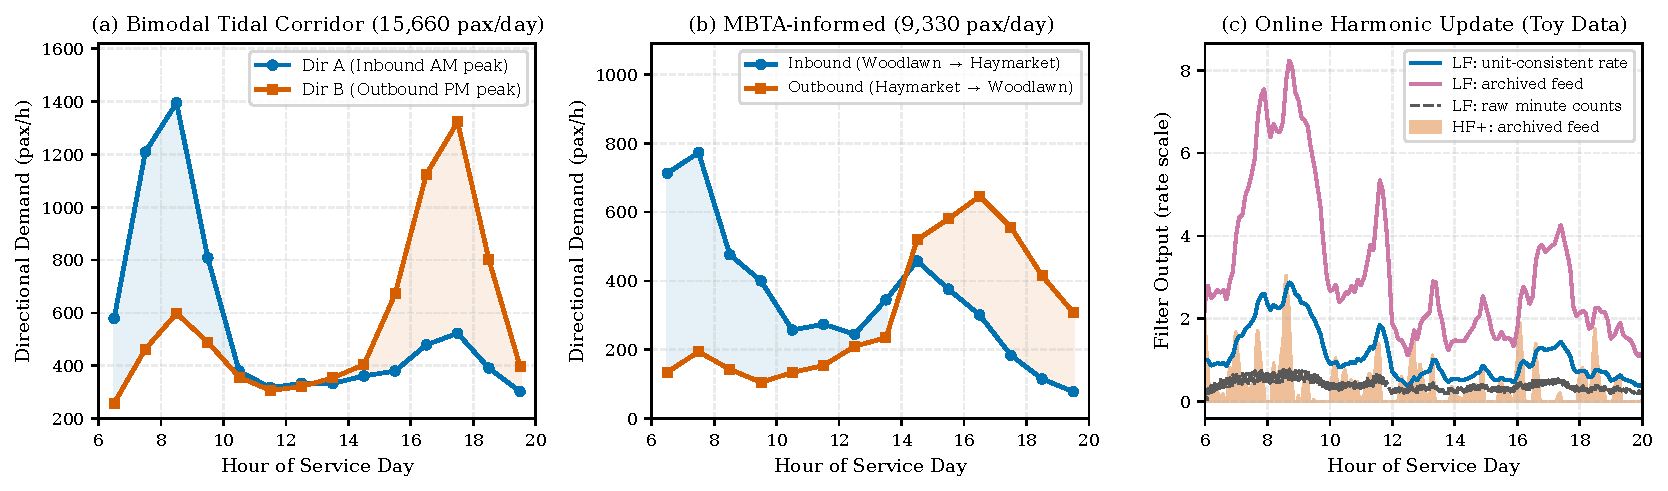
\includegraphics[width=\textwidth]{figures/fig2_corridors_decomposition.pdf}
  \caption{Benchmark corridor demand profiles and causal frequency decomposition: (a) Synthetic Bimodal Tidal Corridor ($15{,}660\text{ pax/day}$, $3.20\times$ peak-to-trough wave with $70/30$ morning/evening reversal); (b) Empirical Fall~2025 Boston MBTA Route~111 weekday corridor ($9{,}330\text{ pax/day}$ across $23$ GTFS stops from Woodlawn to Haymarket, exhibiting $5.3:1$ morning inbound and $3.6:1$ afternoon outbound tidal asymmetries); (c) Illustration of headway-normalized Harmonic-RLS decomposition ($\hat{\lambda}^{\mathrm{LF}}_t$ and $e^+_t$) versus downward Jensen bias under unnormalized $1\text{-min}$ $\log(1+b_t)$ filtering.}
  \label{fig:corridors}
\end{figure}

\begin{enumerate}
  \item \textbf{Bimodal Tidal Corridor (\texttt{Tidal-Bimodal}):} A $20\text{-stop}$ radial corridor ($14{,}400\text{ m}$ one-way) operated by $N_{\mathrm{fleet}} = 14$ standard $12\text{-m}$ urban buses ($C_{\mathrm{bus}} = 75\text{ pax}$) serving an exact daily quota of $262$ trips ($M_+ = M_- = 131$, nominal headway $360\text{ s}$). Mean weekday demand totals $15{,}660\text{ pax/day}$ with a $3.20\times$ bimodal peak-to-trough ratio and strong tidal reversal ($1{,}396\text{ pax/h}$ inbound vs.\ $598\text{ pax/h}$ outbound at $08{:}00$; $523\text{ pax/h}$ inbound vs.\ $1{,}323\text{ pax/h}$ outbound at $17{:}00$; Figure~\ref{fig:corridors}a).

  \item \textbf{Boston MBTA Route~111 Empirical Corridor (\texttt{MBTA-111}):} Reconstructed directly from Fall~2025 Massachusetts Bay Transportation Authority (MBTA) General Transit Feed Specification (GTFS) stop coordinates, inter-stop link distances, scheduled running times, and stop-level weekday APC ridership ($1.35\times$ busy-weekday demand scaling, $9{,}330\text{ pax/day}$). Route~111 connects Woodlawn in Chelsea (\texttt{M01}: Elm St opp.\ Haskell Ave) across the $2{,}880\text{ m}$ Tobin Bridge express span (\texttt{M21}--\texttt{M22}) to Haymarket in Downtown Boston (\texttt{M23}: Surface Rd @ Hanover St), spanning $23$ physical stops and $9{,}069.6\text{ m}$ one-way ($N_{\mathrm{fleet}} = 14$, $C_{\mathrm{bus}} = 75$, $262$ daily trips). As shown in Figure~\ref{fig:corridors}b, Route~111 exhibits extreme asymmetric commuting tides: inbound peak-to-trough reaches $9.91\times$ ($773\text{ pax/h}$ inbound vs.\ $194\text{ pax/h}$ outbound at $07{:}00$), reversing in the afternoon ($646\text{ pax/h}$ outbound vs.\ $301\text{ pax/h}$ inbound at $16{:}00$, $6.15\times$ outbound peak-to-trough).

  \item \textbf{Stationary Flat Corridor (\texttt{Flat-Null}):} A stationary null-check corridor ($N_{\mathrm{fleet}} = 12$, $C_{\mathrm{bus}} = 50$, $262$ trips) with time-invariant arrival rates and zero localized surges, testing whether \texttt{FreqDuet} avoids spurious timetable oscillation when low-frequency modulation offers zero theoretical gain.
\end{enumerate}

\subsection{Baselines, Frequency-Routing Matrix, and Structural Ablations}
\label{sec:setup_baselines}

We benchmark $12$ control methods spanning classical analytical feedback, rolling-horizon economic model predictive control (MPC), single-level DRL, and matched bi-level HRL ablations:
\begin{itemize}
  \item \textbf{\texttt{Fixed-NoHold} ($B_0$):} Nominal $360\text{ s}$ bidirectional schedule with zero stop-level holding ($u_e \equiv 0$).
  \item \textbf{\citet{daganzo2009headway} ($B_1$):} Causal one-sided forward-headway linear feedback $u_e = \mathrm{round}_5(\mathrm{clip}(0.60(H_0 - g^{\mathrm{fwd}}), 0, 20\text{ s}))$.
  \item \textbf{\citet{berrebi2018comparing} ($B_2$):} Causal two-sided bilateral headway equalization $u_e = \mathrm{round}_5(\mathrm{clip}(\frac{1}{2}(g^{\mathrm{bwd}} - g^{\mathrm{fwd}}), 0, 15\text{ s}))$ using same-time AVL follower departure gaps.
  \item \textbf{\texttt{Econ-MPC} ($B_3$):} A rolling-horizon bi-level economic MPC controller that replans quota-conserving headways every $900\text{ s}$ via Newell's square-root rule on trailing $10\text{-min}$ raw APC counts (without Harmonic-RLS decomposition or shock promotion) and optimizes discrete stop holding $u_e \in \{0,\dots,20\}\text{ s}$ via one-step Osuna--Newell net person-seconds maximization within the Turnaround Budget Ledger.
  \item \textbf{\texttt{Flat-SAC} ($B_4$):} Single-level stop-event discrete Ensemble SAC \citep{haarnoja2018soft,christodoulou2019discrete} trained directly on raw APC history without upper slow-clock replanning or turnaround budgeting, representative of single-layer RL holding controllers \citep{alesiani2018rl,wang2020dynamic}.
  \item \textbf{\texttt{NoFreq-HRL} ($B_5$):} Bi-level turnaround-budgeted Constrained Ensemble SAC sharing \texttt{FreqDuet}'s exact architecture, rewards, and $(21, 20)$ state dimensions, but observing only coarse $15\text{-min}$ trailing boarding counts, vehicle load factors, and stop dwell times without frequency decomposition.
  \item \textbf{Four-Way Frequency Routing Matrix:} Keeping network architectures ($96\times 96$ MLPs, $E=6$ critics), dimensions $(21, 20)$, rewards, and turnaround ledger identical, we compare \textbf{\texttt{FreqDuet} (\texttt{Aligned}: $\text{LF}\to\text{U}, \text{HF}\to\text{L}$)} against \textbf{\texttt{Abl-RawHistory}} (trailing multi-window raw APC rates at both levels), \textbf{\texttt{Abl-AllBand}} (unseparated LF, HF, and raw APC concatenated at both levels), and \textbf{\texttt{Abl-Swapped}} (inverted routing: $\text{HF}\to\text{U}, \text{LF}\to\text{L}$).
  \item \textbf{Mechanism Ablations:} \textbf{\texttt{Abl-NoBudget}} disables the Turnaround Budget Ledger ($B_{v,m} \equiv \infty$, removing the hard mask and turnaround shadow guard while keeping aligned frequency features) to test long-horizon training stability; \textbf{\texttt{Abl-NoPromotion}} disables the persistent shock promotion gate ($\eta_{\mathrm{promo}} = 0$) to isolate its contribution under regime shifts.
\end{itemize}

\begin{table}[t]
\centering
\caption{Key physical, estimator, and reinforcement learning hyperparameters (held fixed across all corridors).}
\label{tab:hyperparams}
\resizebox{\textwidth}{!}{%
\begin{tabular}{@{}ll|ll@{}}
\toprule
Parameter & Value & Parameter & Value \\
\midrule
Slow-clock period $\Delta T_U$ & $900\text{ s}$ ($N_U = 6$ backup) & Upper / Lower hidden units & $96 \times 96$ MLP \\
Upper discrete plan set $|\mathcal{A}_U|$ & $5 \times 3 \times 2 = 30$ & Critic ensemble size $E$ & $6$ ($\beta_{\mathrm{LCB}} = -1.0$) \\
Loop factor $\rho_k$ & $\{0.78, 0.89, 1.0, 1.12, 1.24\}$ & Discount factors $(\gamma_U, \gamma_L)$ & $(0.996,\, 0.92)$ \\
Directional tilt $\delta_k$ & $\{-36,\, 0,\, +36\}\text{ s}$ & Learning rates $(\text{actor/critic}, \lambda_L)$ & $(3\times 10^{-4},\, 10^{-3})$ \\
Budget retention $\beta_k$ & $\{0.50,\, 0.90\}$ & Replay capacities $(|\mathcal{D}_U|, |\mathcal{D}_L|)$ & $(20{,}000,\, 180{,}000)$ \\
Lower holding bins $\mathcal{A}_L$ & $\{0, 5, 10, 15, 20, 25\}\text{ s}$ & Updates per episode $(G_U, G_L)$ & $(32,\, 64)$ \\
Harmonic basis order $K$ & $4$ ($P = 50{,}400\text{ s}$) & Lower CMDP cost limit $d_0$ & $0.020$ \\
RLS $(\gamma_f, \sigma_0^2, \tau_{\mathrm{fc}})$ & $(0.998,\, 0.35,\, 20\text{ min})$ & Training horizon $N_{\mathrm{ep}}$ & $200$ service days \\
\bottomrule
\end{tabular}%
}
\end{table}

\subsection{Evaluation Protocol, Common Random Numbers, and Out-of-Distribution Suite}
\label{sec:setup_protocol}

All hyperparameters (Table~\ref{tab:hyperparams}) are locked strictly on disjoint development ($8$ service days) and validation ($10$ service days) cohorts before any evaluation on confirmation scenarios. Training runs span $N_{\mathrm{ep}} = 200$ complete simulated service days per random seed ($6$ independent training seeds in our long-horizon stability audit evaluated at frozen milestones $\text{ep}40$, $\text{ep}100$, and $\text{ep}200$; $4$ independent training seeds across all $8$ learned arms in the full $12$-method confirmation matrix). Every confirmation evaluation uses $16$ untouched CRN service days with synchronized exogenous passenger arrival timestamps, origin--destination draws, link travel-time realizations, and localized demand bursts across all controllers on a given day. We compute $95\%$ confidence intervals on paired day-level differences using $10{,}000$ nonparametric bootstrap resamples over CRN days alongside across-seed standard deviations.

Finally, without retraining any weights, frozen $\text{ep}200$ policies are subjected to four $8\text{-day}$ zero-shot out-of-distribution (OOD) and null stress tests on a separate held-out CRN cohort: (i) \textbf{\texttt{OOD-PeakShift}}, shifting the entire diurnal demand profile by $\pm 1\text{ h}$ on alternating days; (ii) \textbf{\texttt{OOD-HFSurge}}, scaling localized $15\text{-min}$ burst amplitudes by $1.8\times$ ($2.7\times$--$4.3\times$ stop surges); (iii) \textbf{\texttt{OOD-Congestion}}, degrading corridor link speeds by $-0.8\text{ m/s}$ across all segments (tightening fleet-cycle slack toward $H_{\min}$); and (iv) \textbf{\texttt{Null-FlatSanity}}, deploying frozen $14\text{-bus}$ tidal policies zero-shot onto the stationary $12\text{-bus}$ \texttt{Flat-Null} corridor alongside in-domain stationary verification.
